\documentclass{article}\usepackage[]{graphicx}\usepackage[]{color}
%% maxwidth is the original width if it is less than linewidth
%% otherwise use linewidth (to make sure the graphics do not exceed the margin)
\makeatletter
\def\maxwidth{ %
  \ifdim\Gin@nat@width>\linewidth
    \linewidth
  \else
    \Gin@nat@width
  \fi
}
\makeatother

\definecolor{fgcolor}{rgb}{0.345, 0.345, 0.345}
\newcommand{\hlnum}[1]{\textcolor[rgb]{0.686,0.059,0.569}{#1}}%
\newcommand{\hlstr}[1]{\textcolor[rgb]{0.192,0.494,0.8}{#1}}%
\newcommand{\hlcom}[1]{\textcolor[rgb]{0.678,0.584,0.686}{\textit{#1}}}%
\newcommand{\hlopt}[1]{\textcolor[rgb]{0,0,0}{#1}}%
\newcommand{\hlstd}[1]{\textcolor[rgb]{0.345,0.345,0.345}{#1}}%
\newcommand{\hlkwa}[1]{\textcolor[rgb]{0.161,0.373,0.58}{\textbf{#1}}}%
\newcommand{\hlkwb}[1]{\textcolor[rgb]{0.69,0.353,0.396}{#1}}%
\newcommand{\hlkwc}[1]{\textcolor[rgb]{0.333,0.667,0.333}{#1}}%
\newcommand{\hlkwd}[1]{\textcolor[rgb]{0.737,0.353,0.396}{\textbf{#1}}}%
\let\hlipl\hlkwb

\usepackage{framed}
\makeatletter
\newenvironment{kframe}{%
 \def\at@end@of@kframe{}%
 \ifinner\ifhmode%
  \def\at@end@of@kframe{\end{minipage}}%
  \begin{minipage}{\columnwidth}%
 \fi\fi%
 \def\FrameCommand##1{\hskip\@totalleftmargin \hskip-\fboxsep
 \colorbox{shadecolor}{##1}\hskip-\fboxsep
     % There is no \\@totalrightmargin, so:
     \hskip-\linewidth \hskip-\@totalleftmargin \hskip\columnwidth}%
 \MakeFramed {\advance\hsize-\width
   \@totalleftmargin\z@ \linewidth\hsize
   \@setminipage}}%
 {\par\unskip\endMakeFramed%
 \at@end@of@kframe}
\makeatother

\definecolor{shadecolor}{rgb}{.97, .97, .97}
\definecolor{messagecolor}{rgb}{0, 0, 0}
\definecolor{warningcolor}{rgb}{1, 0, 1}
\definecolor{errorcolor}{rgb}{1, 0, 0}
\newenvironment{knitrout}{}{} % an empty environment to be redefined in TeX

\usepackage{alltt}
\IfFileExists{upquote.sty}{\usepackage{upquote}}{}
\begin{document}

\begin{knitrout}
\definecolor{shadecolor}{rgb}{0.969, 0.969, 0.969}\color{fgcolor}\begin{kframe}
\begin{alltt}
\hlstd{SleepingBeauty} \hlkwb{<-} \hlkwa{function}\hlstd{(}\hlkwc{p}\hlstd{) \{}
  \hlstd{a} \hlkwb{<-} \hlnum{0}

  \hlstd{heads} \hlkwb{<-} \hlkwd{sample}\hlstd{(}\hlkwd{c}\hlstd{(}\hlnum{0}\hlstd{,}\hlnum{1}\hlstd{), c1,} \hlnum{TRUE}\hlstd{,} \hlkwd{c}\hlstd{(}\hlnum{1}\hlopt{-}\hlstd{p,p))}
  \hlstd{a} \hlkwb{<-} \hlstd{a} \hlopt{+} \hlkwd{sum}\hlstd{(heads)}

  \hlstd{heads} \hlkwb{<-} \hlkwd{sample}\hlstd{(}\hlkwd{c}\hlstd{(}\hlnum{0}\hlstd{,}\hlnum{1}\hlstd{),} \hlnum{2}\hlopt{*}\hlstd{c2,} \hlnum{TRUE}\hlstd{,} \hlkwd{c}\hlstd{(}\hlnum{1}\hlopt{-}\hlstd{p,p))}
  \hlstd{a} \hlkwb{<-} \hlstd{a} \hlopt{+} \hlnum{2}\hlopt{*}\hlstd{c2}\hlopt{-}\hlkwd{sum}\hlstd{(heads)}

  \hlkwd{return}\hlstd{(a)}
\hlstd{\}}

\hlstd{N} \hlkwb{<-} \hlnum{10000} \hlcom{# Number of experiments}
\hlstd{M} \hlkwb{<-} \hlnum{100}   \hlcom{# Number of tested probabilities}

\hlstd{res} \hlkwb{<-} \hlkwd{vector}\hlstd{(}\hlkwc{length}\hlstd{=M}\hlopt{+}\hlnum{1}\hlstd{)}
\hlstd{coins} \hlkwb{<-} \hlkwd{sort}\hlstd{(}\hlkwd{sample}\hlstd{(}\hlkwd{c}\hlstd{(}\hlnum{0}\hlstd{,}\hlnum{1}\hlstd{), N,} \hlnum{TRUE}\hlstd{))}
\hlstd{c1} \hlkwb{<-} \hlkwd{sum}\hlstd{(coins)}
\hlstd{c2} \hlkwb{<-} \hlstd{N} \hlopt{-} \hlstd{c1}

\hlkwa{for} \hlstd{(i} \hlkwa{in} \hlnum{1}\hlopt{:}\hlstd{(M}\hlopt{+}\hlnum{1}\hlstd{)) \{}
  \hlstd{res[i]} \hlkwb{<-} \hlkwd{SleepingBeauty}\hlstd{((i}\hlopt{-}\hlnum{1}\hlstd{)}\hlopt{/}\hlstd{M)}
\hlstd{\}}

\hlcom{# Average probability of correct guess}
\hlstd{resProb} \hlkwb{<-} \hlstd{res} \hlopt{/} \hlstd{(c1} \hlopt{+} \hlnum{2}\hlopt{*}\hlstd{c2)}

\hlkwd{plot}\hlstd{(}\hlkwd{seq}\hlstd{(}\hlnum{0}\hlstd{,}\hlnum{1}\hlstd{,}\hlnum{1}\hlopt{/}\hlstd{M), resProb,} \hlkwc{xlab}\hlstd{=}\hlstr{'Probability of guessing heads'}\hlstd{,}
     \hlkwc{ylab}\hlstd{=}\hlstr{'Probability of guessing correctly'}\hlstd{,}
     \hlkwc{main}\hlstd{=}\hlstr{'Probability of guessing correctly in Sleeping Beauty'}\hlstd{)}
\hlkwd{abline}\hlstd{(}\hlnum{2}\hlopt{/}\hlnum{3}\hlstd{,}\hlopt{-}\hlnum{1}\hlopt{/}\hlnum{3}\hlstd{,} \hlkwc{col}\hlstd{=}\hlstr{'red'}\hlstd{)}
\end{alltt}
\end{kframe}
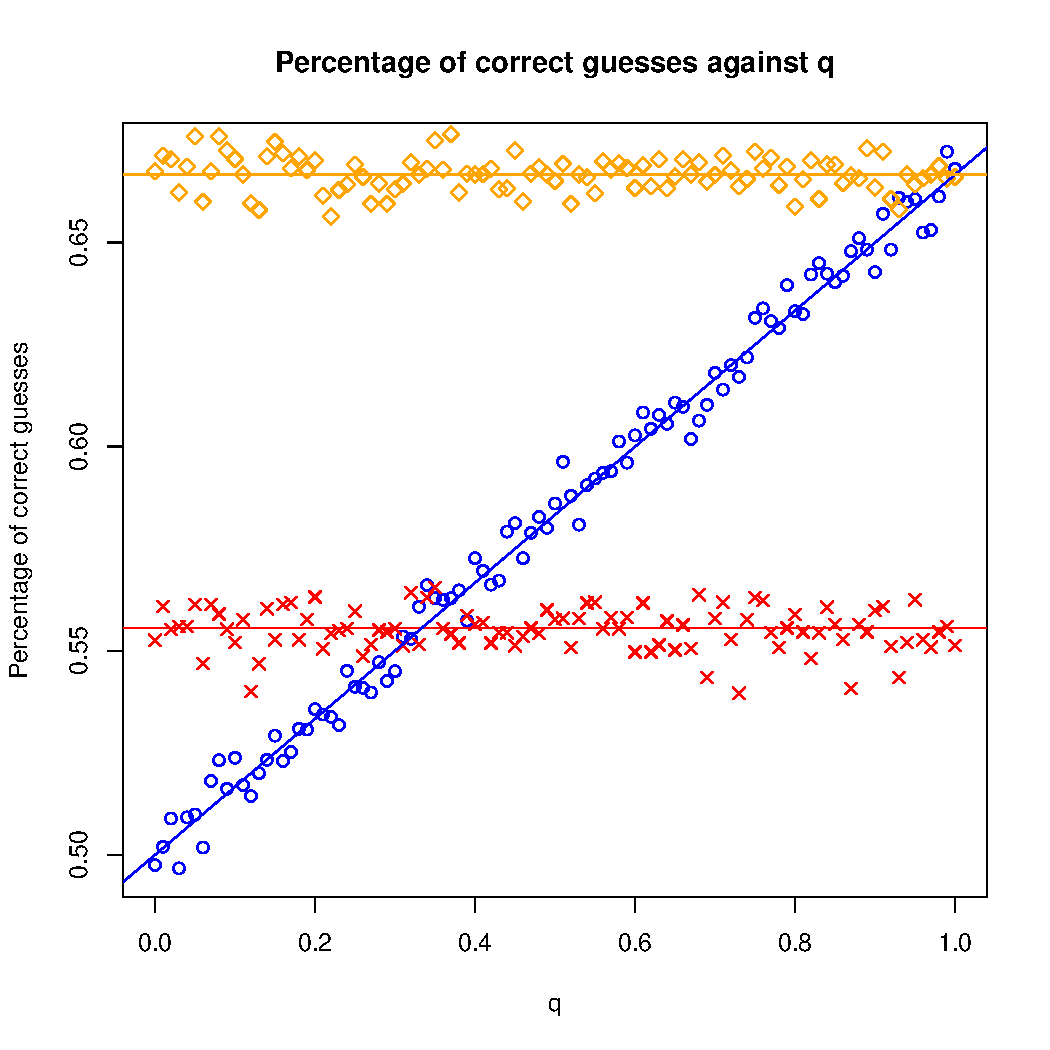
\includegraphics[width=\maxwidth]{figure/unnamed-chunk-1-1} 

\end{knitrout}


\end{document}
